\documentclass[11pt,a4paper,oneside]{article}
\usepackage[latin1]{inputenc}
\usepackage{amsmath}
\usepackage{amsfonts}
\usepackage{amssymb}
\usepackage{graphicx}
\usepackage{color}
\usepackage {tikz}
\usetikzlibrary {er}
\usepackage[left=2.00cm, right=2.00cm, top=1.00cm]{geometry}
\graphicspath{{./}}

\begin{document}
	\title{DS 221 - Introduction to Scalable Systems \\ Assignment 2}
	\author{Shriram R. \\ M Tech (CDS) \\ 06-02-01-10-51-18-1-15763}
	\maketitle
	
	\section{2D Matrices}
	The 2D matrix abstract data structure has been implemented using 2D array and compressed sparse matrix representation (CSR) and the space and time complexities has been analyzed and empirically verified.
	The following sections will cover the analysis and empirical results in detail.
	
	\subsection{Storage Space}
	Let N, M and NNZ denote the number of rows, columns and non-zero elements of the matrix respectively. This notation will be used for the remainder of the report. For 2D array implementation, space is allocated to each element irrespective of the value and so the asymptotic space complexity is O(NM). \\
	\newline
	For CSR implementation, we have three 1D arrays namely A for storing matrix values, IA for storing the cumulative sum of non-zero values for each row and JA for string the column index for each non-zero value. These array have NNZ, N+1 and NNZ elements respectively. Hence, the asymptotic space complexity is O(N + 2NNZ)  \\
	\newline
	The space complexities has been empirically determined for various matrix sizes and sparsities and the results are provided below. Square matrices (N=M) were used for simplicity of analysis,
	
	\begin{center}
		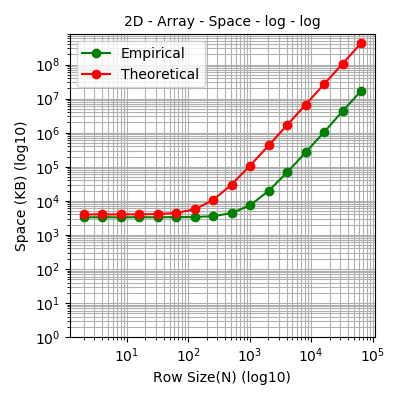
\includegraphics[scale=0.6]{1.png}		
	\end{center}

	\begin{center}
		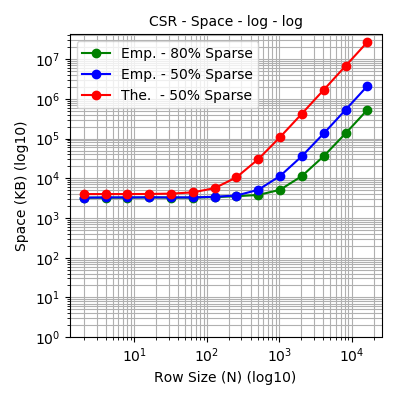
\includegraphics[scale=0.6]{2.png}		
	\end{center}

    \subsection{Matrix Addition}
    For matrix addition, all the elements of the input and output matrices have to be processed exactly once and there are NM elements in each matrix. \\
    \newline
    In the case of 2D array implementation, each element can be accessed in $O(1)$ time and so the total time complexity for addition in this case is $O(NM)$. \\
    \newline
    For the case of CSR implementation, each element can be accessed in $O(M)$ time assuming the worst case where a row has all the elements as non-zero. So, the time complexity for addition in this case will be $O(NM^2)$. \\   
    \newline
    The time complexities has been empirically determined for various matrix sizes and sparsities and the results are provided below. Square matrices (N=M) were used for simplicity of analysis,
    
    \begin{center}
    	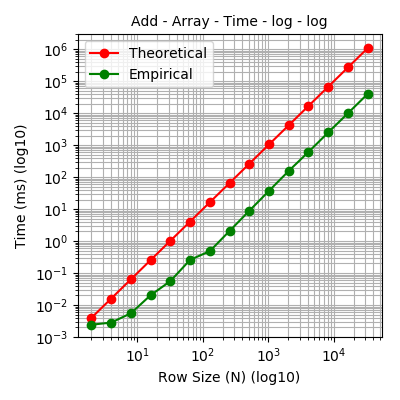
\includegraphics[scale=0.6]{3.png}		
    \end{center}
    
    \begin{center}
    	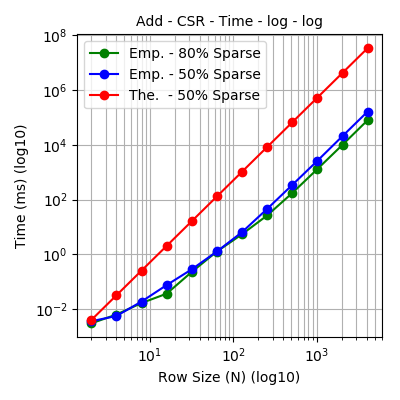
\includegraphics[scale=0.6]{4.png}		
    \end{center}
    
    \subsection{Matrix Multiplication}
    For matrix multiplication, naive or brute force implementation takes $O(N^3)$ multiplication and addition operations for multiplying two NxN square matrices. \\
    \newline
    In the case of 2D array implementation, each element can be accessed in $O(1)$ time and so the total time complexity for addition in this case is $O(N^3)$. \\
    \newline
    For the case of CSR implementation, each element can be accessed in $O(N)$ time assuming the worst case where a row has all the elements as non-zero. So, the time complexity for addition in this case will be $O(N^4)$. \\   
    \newline    
    The time complexities has been empirically determined for various matrix sizes and sparsities and the results are provided below,
    
     \begin{center}
    	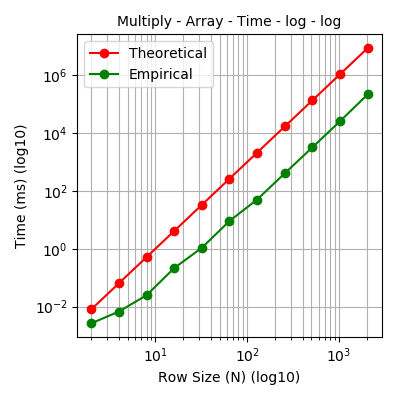
\includegraphics[scale=0.6]{5.png}		
    \end{center}
    
    \begin{center}
    	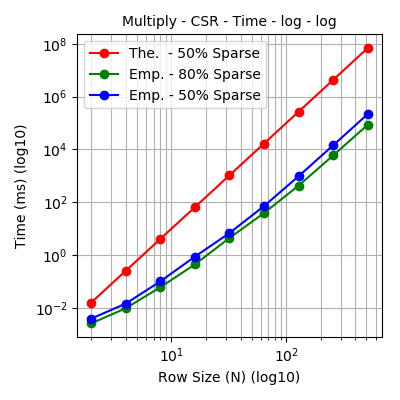
\includegraphics[scale=0.6]{6.png}		
    \end{center}

    \subsection{Breadth First Search}
    
    The time complexity of Breadth first search is O(V+E) where V is the no. of nodes and E is the no. of edges

    \section{Conclusion}
    It has been observed that the cache optimized and vectorized version of the program performs significantly better and scales well with the size of matrix. The optimized version took $0.513s$ to multiply 1024x1024 matrices of \emph{double} items. It is possible to improve the performance further by using divide and conquer algorithm like Strassen's which has a better complexity than $O(n^3)$. 
    
    \section{References}
    
    \begin{list}{*}{}
    	\item https://gcc.gnu.org/projects/tree-ssa/vectorization.html
    	\item https://stackoverflow.com/questions/1847789/segmentation-fault-on-large-array-sizes
    	\item https://linux.die.net/man/3/clock\_gettime
    	\item DS 221 Course lecture notes
    \end{list}

\end{document}